\documentclass[11pt]{article}

\usepackage[T1]{fontenc}
\usepackage[utf8]{inputenc}
\usepackage{lmodern}
\usepackage{microtype}
\usepackage{geometry}
\usepackage{amsmath,amssymb,bm}
\usepackage{booktabs}
\usepackage{array}
\usepackage{graphicx}
\usepackage{caption}
\usepackage{subcaption}
\usepackage{xcolor}
\usepackage{hyperref}
\usepackage[numbers,sort&compress]{natbib}
\usepackage{enumitem}

\geometry{margin=1in}
\hypersetup{
  colorlinks=true,
  linkcolor=blue!55!black,
  citecolor=blue!55!black,
  urlcolor=blue!55!black
}
\newcommand{\phidir}{\Phi_{\mathrm{dir}}}
\newcommand{\phirot}{\Phi_{\mathrm{rot}}}
\newcommand{\phitan}{\Phi_{\mathrm{tan}}}
\newcommand{\lbar}{\overline{L}}
\newcommand{\vrbar}{\overline{v}_{r}}
\newcommand{\sigmad}{\sigma_d}

\title{\textbf{From Simulated Collective Dynamics to Real Fish-School Motion Classification:}\\
An Order-Parameter-Based Pipeline}

\author{
  Josef Berman\\
  School of Marine Sciences, University of Haifa, Haifa, Israel\\
  \texttt{[corresponding-author email]}
}

\date{}

\begin{document}
\maketitle

\begin{abstract}
Automatically identifying collective motion regimes from tracked animal trajectories is useful for
studying transitions, perturbation responses, and group-level decision making, but labelled biological
data are typically scarce and imbalanced. We present an end-to-end pipeline that generates synthetic
fish-school trajectories, summarizes them with interpretable collective order parameters, and trains a
multiclass motion classifier. Six regimes are represented: polarized travelling, milling, swarming,
fountain evasion, expansion burst, and compaction. A continuous bounded-turning simulator combines
short-range repulsion, alignment, attraction, confinement, and regime-specific threat dynamics.
For each trajectory we aggregate directional polarization, normalized angular momentum, rotational
polarization, tangential order, signed radial motion, and radial spread into 15 segment-level features.
A histogram-based gradient-boosting classifier is trained only on accepted simulations and evaluated
on held-out random seeds and on manually annotated real trajectories. Of 3,600 intended simulations,
3,552 passed the behaviour-specific validation filters and entered the classifier dataset. On 711
held-out simulated clips, the model achieved 98.17\% accuracy and 98.18\% macro-F1. In contrast, on
115 real segments from ten recordings, accuracy was 37.39\% and macro-F1 was 33.24\%. The largest
error mode was systematic overprediction of expansion bursts. These results show that low-dimensional
order parameters can sharply separate regimes generated by the simulator, while also exposing a
substantial simulation-to-reality domain gap. The pipeline therefore provides a reproducible baseline
and a diagnostic framework, rather than evidence that simulation-only training is sufficient for
deployment on biological data.
\end{abstract}

\noindent\textbf{Keywords:} collective motion; fish schooling; order parameters; agent-based simulation;
gradient boosting; sim-to-real transfer; behaviour classification

\section{Introduction}

Fish schools exhibit structured collective states that emerge from local interactions among individuals.
Classical self-propelled-particle models show that changes in repulsion, orientation, and attraction can
produce qualitatively different group configurations \citep{couzin2002}. Empirical work has likewise
shown that schooling fish occupy macroscopic regimes such as swarming, milling, and polarized motion,
and that transitions among these regimes can be summarized by a small number of collective order
parameters \citep{tunstrom2013}. Data-driven models further demonstrate that social-response functions,
confinement, speed, and group size jointly shape the phase diagram of collective motion
\citep{gautrais2012,calovi2014}.

The standard stable regimes do not exhaust the behavioural repertoire. Under threat, a school may split
around an approaching predator and reunite in a fountain manoeuvre \citep{hall1986}, rapidly expand
following a propagated startle response, or compact by reducing inter-individual spacing. These
transient events are scientifically important but difficult to classify: they are short, rare in
observational data, and often embedded within longer baseline periods.

Supervised learning from real trajectories is constrained by limited annotations, heterogeneous tracking
quality, and severe class imbalance. Simulation offers an attractive source of labelled examples, but
synthetic labels are meaningful only when the generator produces realistic within-class variability and
when performance transfers beyond the simulator. A nearly perfect synthetic holdout score can otherwise
measure recovery of simulator settings rather than biological generalization.

This work develops and evaluates the \textit{SchoolMotionClassifier} pipeline. Its contributions are:

\begin{enumerate}[leftmargin=*]
  \item an agent-based simulator spanning three stable and three threat-induced collective regimes;
  \item a common trajectory schema for synthetic and real data;
  \item a compact, interpretable 15-dimensional representation derived from six order-parameter time
  series;
  \item a seed-disjoint synthetic evaluation and an external evaluation on manually annotated real
  trajectory segments; and
  \item an explicit analysis of the resulting simulation-to-reality gap.
\end{enumerate}

\section{Materials and Methods}

\subsection{Problem formulation}

Each observation is a planar multi-agent trajectory
\(\mathcal{T}=\{(\bm{x}_i(t),\bm{v}_i(t))\}_{i=1}^{N}\), where
\(\bm{x}_i(t)\in\mathbb{R}^{2}\) and \(\bm{v}_i(t)\in\mathbb{R}^{2}\) are the
position and velocity of fish \(i\) at frame \(t\). The objective is to assign one of six canonical
labels:
\[
\mathcal{Y}=\{\text{polarized},\text{milling},\text{swarming},
\text{fountain},\text{expansion},\text{compaction}\}.
\]
The implementation uses the longer identifiers \texttt{traveling\_polarized},
\texttt{fountain\_evasion}, and \texttt{expansion\_burst}. Alias resolution maps annotation terms such
as \texttt{polarized}, \texttt{burst}, \texttt{spread}, and \texttt{contraction} to the canonical set.

\subsection{Trajectory data}

\subsubsection{Synthetic design}

The factorial design contains six behaviours, six group sizes
\(N\in\{10,20,30,40,100,200\}\), and 100 nominal random seeds, for 3,600 intended
clips. Seeds 0--79 form the training partition and seeds 80--99 form the test partition. This split
prevents the same stochastic realization from occurring on both sides of the evaluation. Each accepted
clip contains 450 frames at 30 frames per second after a behaviour-specific burn-in of 80--150 frames.
Stable behaviours are represented by the full clip. Threat behaviours use fixed event-focused intervals:
frames 100--300 for fountain evasion, 120--260 for expansion burst, and 120--320 for compaction.

Generation applies up to four attempts per design point. A behaviour-specific validation gate determines
whether a realization has the intended qualitative signature. If all attempts fail, the final realization
is stored with \texttt{valid=false} and excluded from model fitting and evaluation. The resulting feature
dataset contains 2,841 training and 711 test clips (3,552 accepted in total).

\subsubsection{Real trajectory segments}

The repository defines ten recordings at 29.97 frames per second, with group-size directories for
10, 30, 70, and 150 fish. Manual annotations provide start time, end time, and raw behaviour label.
Segments shorter than 0.5 seconds are excluded. The evaluation set contains 115 retained segments:
62 polarized, 36 milling, 12 swarming, one fountain, and four expansion-burst segments. No real
compaction annotation is available, so compaction is excluded from real-data metrics. The trajectory
files themselves are intentionally not versioned in the repository; the analysis expects comma-separated
files containing a frame column and per-fish \(x,y,v_x,v_y\) columns.

\paragraph{Provenance limitation.}
The current repository records frame rate, group-size folder, and manual segment annotations but does
not encode species, experimental protocol, tracking uncertainty, licensing, or a permanent identifier
for the real trajectory source. These fields must be added before archival publication. Accordingly,
the real-data experiment is described here as an external pilot evaluation rather than a fully
reproducible biological benchmark.

\subsection{Agent-based school simulator}

\subsubsection{State and motion update}

Each simulated fish has position \(\bm{x}_i\), heading \(\theta_i\), scalar speed \(s_i\), preferred
spacing \(d_{0,i}\), and a discrete state \(q_i\). Its heading vector is
\(\bm{h}_i=(\cos\theta_i,\sin\theta_i)\), so the position update is
\begin{equation}
  \bm{x}_i(t+\Delta t)=\bm{x}_i(t)+s_i(t+\Delta t)\bm{h}_i(t+\Delta t)\Delta t.
\end{equation}
The frame-based implementation uses \(\Delta t=1\), with position and velocity expressed in pixels and
pixels per frame. Speed relaxes toward a state-dependent target \(s_i^\star\):
\begin{equation}
  a_i(t)=\operatorname{clip}\!\left(
  \frac{s_i^\star(t)-s_i(t)}{\tau_s},-a_{\max},a_{\max}\right),
  \qquad
  s_i(t+\Delta t)=\operatorname{clip}\!\left(s_i(t)+a_i(t)\Delta t,
  s_{\min},1.2s_{\mathrm{escape}}\right).
\end{equation}

The angular velocity is a clipped weighted sum of repulsion, orientation, attraction, wall, predator,
and circulation torques:
\begin{equation}
  \omega_i=\operatorname{clip}\!\left(
  w_{r,i}T_{r,i}+w_{o,i}T_{o,i}+w_{a,i}T_{a,i}
  +T_{w,i}+w_{p,i}T_{p,i}+T_{c,i}+\epsilon_i,
  -\omega_{\max},\omega_{\max}\right),
\end{equation}
\begin{equation}
  \theta_i(t+\Delta t)=\left[\theta_i(t)+\omega_i(t)\Delta t\right]\bmod 2\pi,
  \qquad \epsilon_i\sim\mathcal{N}(0,\sigma_\theta^2).
\end{equation}

\subsubsection{Local social interactions and confinement}

Although the repository also contains a slower Voronoi-neighbour reference implementation, the bulk
dataset generator calls the optimized simulator. That implementation uses the \(k\) nearest neighbours,
with \(k=\min(8,\max(3,N-1))\). Neighbours in a \(30^\circ\) rear blind region are ignored. The
neighbour list is refreshed every frame for \(N\leq40\) and every third frame for larger schools.
Within this local set, agents turn away from neighbours inside the repulsion/preferred-spacing zone,
align with neighbours inside the orientation radius, and turn toward neighbours between the preferred
spacing and attraction radius. A soft circular wall applies an inward torque near the arena boundary.
The default arena is centred at \((1100,750)\) pixels with radius 420 pixels; milling uses radius
360 pixels and stronger confinement.

\subsubsection{Behaviour parameterization}

Table~\ref{tab:behaviour-configs} summarizes the frozen configuration values that most directly separate
the regimes. All configurations use continuous bounded turning; differences arise from social weights,
noise, speed, circulation, and threat-state modifications.

\begin{table*}[t]
\centering
\caption{Principal simulator parameters by behaviour. Distances are in pixels and speed in pixels per
frame. \(w_r,w_o,w_a\) denote repulsion, orientation, and attraction weights.}
\label{tab:behaviour-configs}
\small
\begin{tabular}{lrrrrrrrr}
\toprule
Behaviour & \(w_r\) & \(w_o\) & \(w_a\) & \(\sigma_\theta\) &
\(\omega_{\max}\) & \(s_{\mathrm{cruise}}\) & \(d_0\) & Special mechanism\\
\midrule
Polarized travelling & 1.8 & 3.2 & 0.55 & 0.05 & 0.40 & 0.95 & 24 & strong alignment\\
Milling              & 1.4 & 0.9 & 2.20 & 0.08 & 0.55 & 0.70 & 32 & \(w_c=1.2\)\\
Swarming             & 2.0 & 0.05& 1.60 & 0.55 & 0.70 & 0.45 & 34 & weak alignment\\
Fountain evasion     & 1.6 & 2.6 & 1.00 & 0.08 & 0.55 & 0.90 & 24 & crossing predator\\
Expansion burst      & 1.6 & 1.6 & 0.70 & 0.10 & 0.60 & 0.85 & 24 & excitable startle\\
Compaction           & 1.4 & 0.8 & 1.50 & 0.15 & 0.45 & 0.65 & 40 & shrinking \(d_0\)\\
\bottomrule
\end{tabular}
\end{table*}

For milling, tangential headings and a circulation torque create coherent rotation. Seeds divisible by
five initialize approximately half the agents in the opposite rotational direction, reduce cross-stream
alignment, and lower the circulation weight to represent bidirectional milling.

For fountain evasion, a predator crosses the arena at 3.5 pixels per frame for 160 frames. Fish inside a
180-pixel response radius turn away at a side-dependent \(40^\circ\) escape angle. Predator torque
receives weight 8.0, while attraction and alignment are temporarily reduced to 70\% and 50\% of their
baseline values.

For expansion bursts, a latent excitation \(z_i\) decays with time constant \(\tau_z\) and increases in
response to the predator and excited neighbours. Crossing threshold \(z_{\mathrm{thr}}\) switches an
agent into a startle state, raises its target speed, triples repulsion, reduces attraction and alignment
to 10\%, and turns it outward from the school centroid. The implementation seeds the whole school
above threshold at event onset; consequently, this version represents a synchronized burst more strongly
than a spatially gradual cascade.

For compaction, the preferred spacing decreases exponentially:
\begin{equation}
 d_{0,i}(t)=\max\!\left(8,d_{0,\mathrm{base}}-\Delta d_0
 \left[1-\exp\!\left(-\frac{t-t_0}{\tau_c}\right)\right]\right),
\end{equation}
with \(\Delta d_0=22\) pixels. Attraction is multiplied by 2.2, alignment by 0.5, repulsion by 0.7,
and target speed by 0.6. After each event, parameters return geometrically toward baseline with update
coefficient 0.08.

\subsection{Collective order parameters}

Let \(\overline{\bm{x}}=N^{-1}\sum_i\bm{x}_i\),
\(\bm{r}_i=\bm{x}_i-\overline{\bm{x}}\), \(r_i=\|\bm{r}_i\|\),
\(\widehat{\bm{r}}_i=\bm{r}_i/r_i\),
\(\widehat{\bm{v}}_i=\bm{v}_i/\|\bm{v}_i\|\), and
\(\widehat{\bm{t}}_i=(-r_{i,y},r_{i,x})/r_i\). Zero-norm cases contribute zero.
Six quantities are computed at every frame:

\paragraph{Directional polarization.}
\begin{equation}
 \phidir=\left\|\frac{1}{N}\sum_{i=1}^{N}\widehat{\bm{v}}_i\right\|.
\end{equation}
Values near one indicate common heading; values near zero indicate directional disorder.

\paragraph{Normalized signed angular momentum.}
\begin{equation}
 L_i=r_{i,x}v_{i,y}-r_{i,y}v_{i,x},\qquad
 \lbar=\frac{N^{-1}\sum_i L_i}{N^{-1}\sum_i r_i}.
\end{equation}
Its sign identifies rotation direction, while its magnitude captures coherent circulation.

\paragraph{Rotational polarization.}
\begin{equation}
 \phirot=\frac{\left|\sum_i L_i\right|}{\sum_i|L_i|}.
\end{equation}
This distinguishes unidirectional rotation from balanced opposing circulation.

\paragraph{Tangential order.}
\begin{equation}
 \phitan=\frac{1}{N}\sum_i
 \left|\widehat{\bm{v}}_i\cdot\widehat{\bm{t}}_i\right|.
\end{equation}
High values indicate motion tangent to the centroid-centred radial direction.

\paragraph{Signed radial motion.}
\begin{equation}
 \vrbar=\frac{1}{N}\sum_i
 \widehat{\bm{v}}_i\cdot\widehat{\bm{r}}_i.
\end{equation}
Positive values indicate outward motion and negative values inward motion. Despite the velocity notation,
this implemented feature is a mean radial direction cosine and is therefore dimensionless.

\paragraph{Radial spread.}
\begin{equation}
 \sigmad=\operatorname{std}_i(r_i).
\end{equation}
This measures heterogeneity of distance from the group centroid, not total school radius or density.

For each series \(g(t)\), segment-level mean and standard deviation are computed. Three additional
features are the least-squares slope of \(\sigmad(t)\), the slope of \(\vrbar(t)\), and
\(\operatorname{mean}_t|\lbar(t)|\), producing 15 classifier inputs. Slopes use time in seconds.
The representation is related to the macroscopic order-parameter approach used to identify stable
states in golden shiner schools \citep{tunstrom2013}, but adds transient radial and spread descriptors.

\subsection{Validation gates}

Soft validation tests reject simulations whose signatures do not match the requested class. Polarized
clips require \(\phidir>0.48\) and \(|\lbar|<0.50\); milling requires sufficient tangential order and
low-to-moderate polarization with evidence of unidirectional or balanced bidirectional rotation; and
swarming requires \(\phidir<0.60\) and \(|\lbar|<0.45\). Threat-regime validation compares pre-event
and event windows. Fountain clips must increase spread by more than one pixel or reduce polarization by
more than 0.05. Expansion clips must increase spread by more than 1.5 pixels or reach radial motion above
0.08. Compaction clips must decrease mean radius by more than two pixels or reduce spread by more than
0.8 pixels. Validation is therefore part of the synthetic data-generating process and should not be
interpreted as an independent test.

\subsection{Classifier and evaluation}

A \texttt{HistGradientBoostingClassifier} is fitted with maximum tree depth 6, learning rate 0.08,
200 boosting iterations, and random seed 42. Gradient boosting constructs an additive ensemble by
stagewise optimization \citep{friedman2001}; the implementation uses scikit-learn
\citep{pedregosa2011}. No hyperparameter search, feature scaling, real-data fine-tuning, probability
calibration, or class reweighting is performed.

Performance is summarized by accuracy, per-class precision, recall and F1, macro-F1, and confusion
matrices. Synthetic metrics include all six classes. Real-data metrics include the five observed classes
and exclude compaction. Because the real class distribution is strongly imbalanced, macro-F1 is treated
as a primary complement to accuracy.

\section{Results}

\subsection{Synthetic holdout performance}

The validation gates retained 3,552 of 3,600 intended simulations (98.67\%): 2,841 training clips and
711 seed-disjoint test clips. The classifier achieved 0.9817 accuracy and 0.9818 macro-F1 on the test
partition. Table~\ref{tab:sim-results} gives class-level results. All 120 swarming and 120 expansion
clips were classified correctly. Fountain evasion was the least precise class (0.9286), mainly because
several polarized, milling, and compaction clips were assigned to fountain. Fountain recall remained
high (0.9832).

\begin{table}[t]
\centering
\caption{Held-out simulated test performance.}
\label{tab:sim-results}
\small
\begin{tabular}{lrrrr}
\toprule
Class & Precision & Recall & F1 & Support\\
\midrule
Polarized travelling & 1.000 & 0.958 & 0.979 & 120\\
Milling              & 1.000 & 0.965 & 0.982 & 115\\
Swarming             & 1.000 & 1.000 & 1.000 & 120\\
Fountain evasion     & 0.929 & 0.983 & 0.955 & 119\\
Expansion burst      & 0.984 & 1.000 & 0.992 & 120\\
Compaction           & 0.983 & 0.983 & 0.983 & 117\\
\midrule
Macro average        & 0.983 & 0.982 & 0.982 & 711\\
\bottomrule
\end{tabular}
\end{table}

\begin{figure}[t]
\centering
\IfFileExists{../results/sim_confusion.png}{
  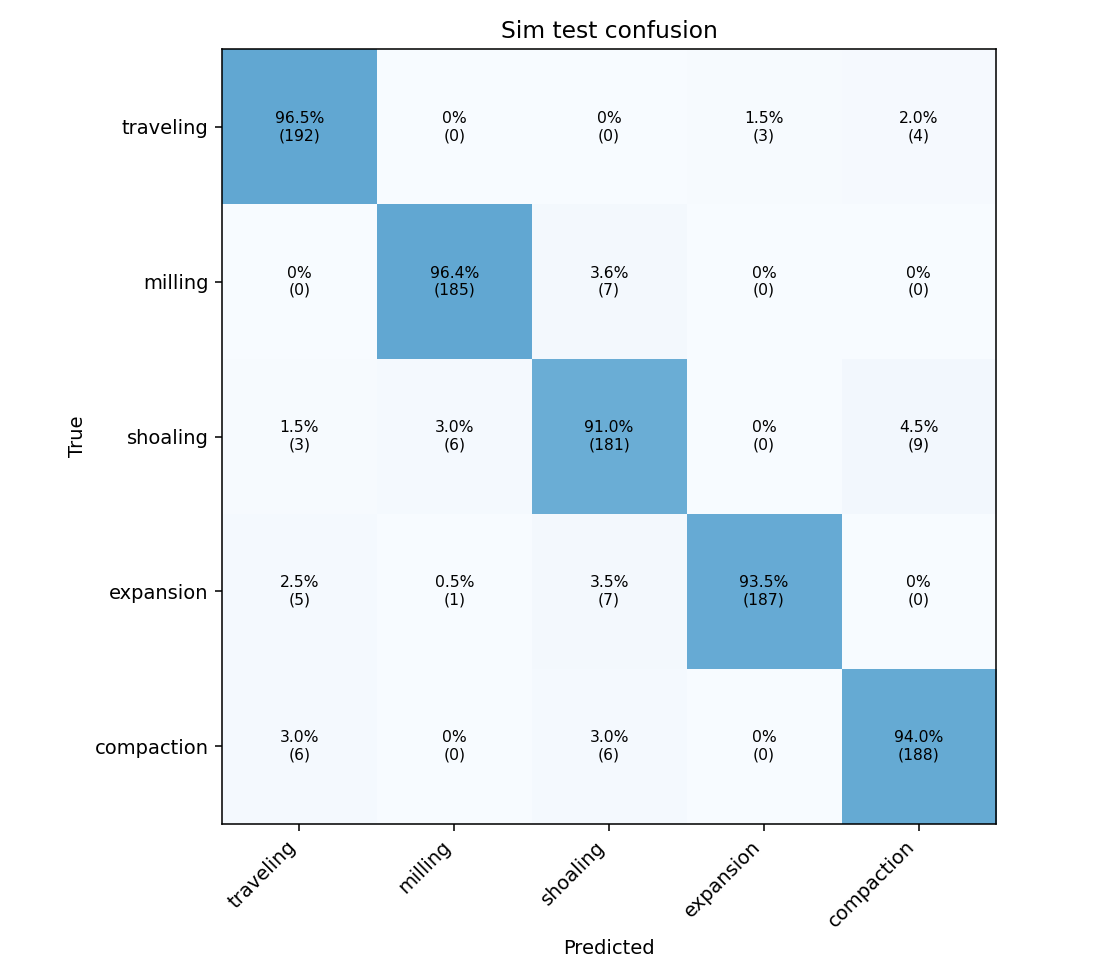
\includegraphics[width=0.82\linewidth]{../results/sim_confusion.png}
}{
  \fbox{\parbox[c][4cm][c]{0.8\linewidth}{\centering
  Missing file: \texttt{results/sim\_confusion.png}}}
}
\caption{Confusion matrix for the seed-disjoint simulated test set.}
\label{fig:sim-confusion}
\end{figure}

\subsection{External real-data evaluation}

Performance dropped substantially on the 115 real segments: accuracy was 0.3739 and macro-F1 was
0.3324. Table~\ref{tab:real-results} shows that milling transferred best (F1 0.6207), followed by
swarming (0.5000) and polarized travelling (0.4304). The single fountain example was missed. All four
expansion examples were detected, but expansion precision was only 0.0588.

\begin{table}[t]
\centering
\caption{Performance on manually annotated real trajectory segments.}
\label{tab:real-results}
\small
\begin{tabular}{lrrrr}
\toprule
Class & Precision & Recall & F1 & Support\\
\midrule
Polarized travelling & 1.000 & 0.274 & 0.430 & 62\\
Milling              & 0.818 & 0.500 & 0.621 & 36\\
Swarming             & 1.000 & 0.333 & 0.500 & 12\\
Fountain evasion     & 0.000 & 0.000 & 0.000 & 1\\
Expansion burst      & 0.059 & 1.000 & 0.111 & 4\\
\midrule
Macro average        & 0.575 & 0.422 & 0.332 & 115\\
\bottomrule
\end{tabular}
\end{table}

The confusion matrix identifies a dominant failure mode: 42 of 62 polarized, 16 of 36 milling, five of
12 swarming, and the only fountain segment were predicted as expansion. In total, 68 of 115 real
segments (59.13\%) received the expansion label. The model was therefore not merely less accurate on
real data; its decision boundary was systematically displaced toward a single transient synthetic class.

\begin{figure}[t]
\centering
\IfFileExists{../results/real_confusion.png}{
  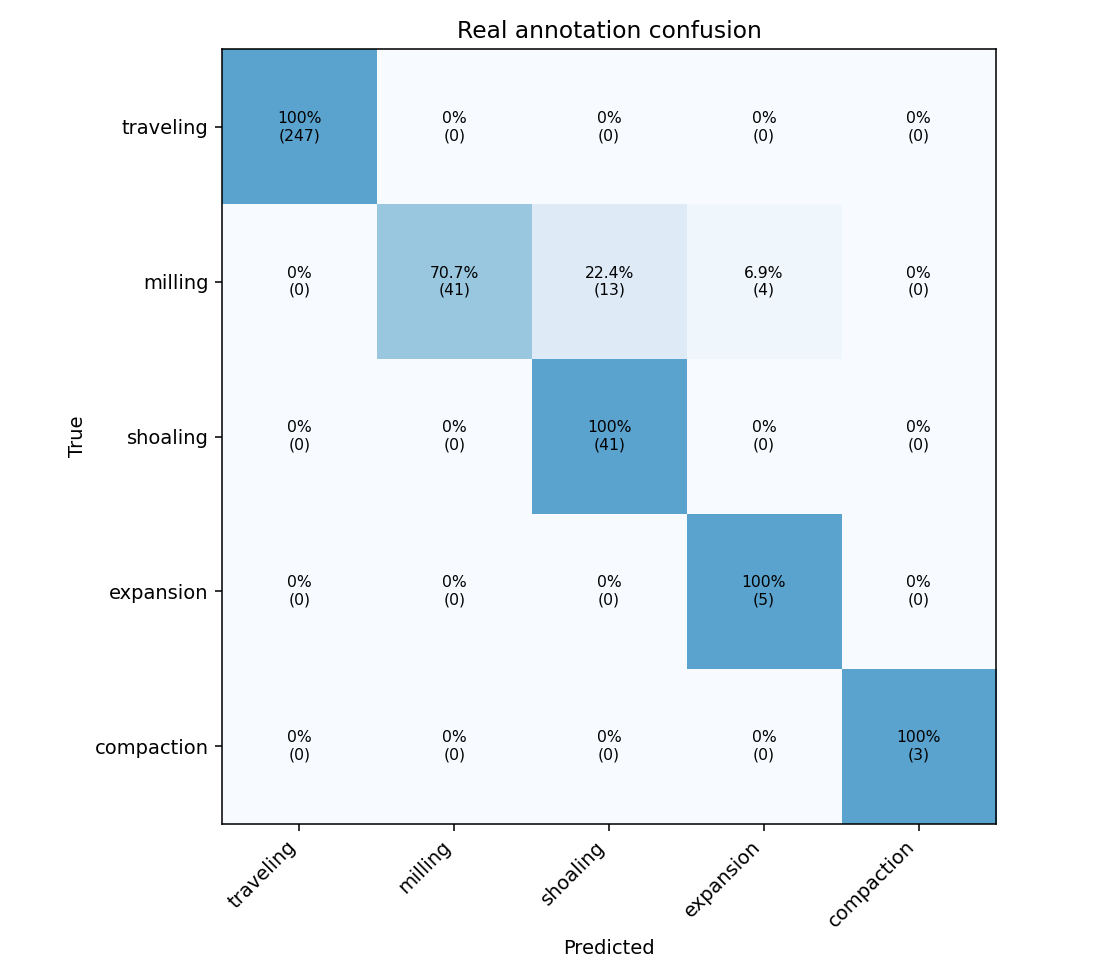
\includegraphics[width=0.82\linewidth]{../results/real_confusion.png}
}{
  \fbox{\parbox[c][4cm][c]{0.8\linewidth}{\centering
  Missing file: \texttt{results/real\_confusion.png}}}
}
\caption{Confusion matrix for the manually annotated real segments. Compaction is excluded because no
real compaction annotation is available.}
\label{fig:real-confusion}
\end{figure}

\section{Discussion}

\subsection{What the synthetic score demonstrates}

The synthetic evaluation demonstrates that the selected order parameters encode the regimes produced by
the simulator with little ambiguity across unseen seeds and across group sizes from 10 to 200. This is a
useful result: the feature representation compresses variable-size trajectories into a fixed
15-dimensional vector while retaining interpretable cues for alignment, rotation, radial motion, and
spread. The high score also confirms that transient-event windows and stable full-clip segments can be
handled by the same tabular model.

However, the result is conditional on the generator and its validation filters. Behaviour configurations
change several factors simultaneously, including noise, speed, attraction, alignment, confinement, and
event timing. The classifier may thus learn parameter-set fingerprints that are more separable than
biological states. Moreover, rejected simulations are removed before training and testing, narrowing
within-class variability. The 98\% synthetic accuracy should be interpreted as internal pipeline
consistency, not as an estimate of real-world behaviour-recognition performance.

\subsection{Sources of the simulation-to-reality gap}

Several mechanisms plausibly explain the external failure:

\begin{enumerate}[leftmargin=*]
  \item \textbf{Feature-scale mismatch.} Five features are dimensionless, but \(\lbar\), \(\sigmad\),
  and the spread slope depend on coordinate and velocity scale. No normalization by body length, arena
  size, median inter-individual distance, or trajectory-specific scale is applied.
  \item \textbf{Simulator-induced radial bias.} The calibration report contains strongly negative mean
  radial-direction cosines even for nominally stable polarized, milling, and swarming clips. This suggests
  that confinement and attraction produce systematic inward motion, complicating the intended
  interpretation of \(\vrbar\) as a transient expansion/compaction cue.
  \item \textbf{Synchronized synthetic expansion.} At startle onset, all simulated agents are forced
  above the excitation threshold. The expansion class may consequently occupy an unrealistically broad
  or shifted region in feature space.
  \item \textbf{Event-window asymmetry.} Synthetic threat clips are cropped to known event windows,
  whereas real annotations vary widely in duration and may contain onset, recovery, or mixed states.
  \item \textbf{Local-interaction approximation.} Bulk simulations use cached \(k\)-nearest-neighbour
  graphs, rather than the Voronoi neighbourhoods described in the reference implementation. This choice
  improves throughput but may change density- and group-size-dependent dynamics.
  \item \textbf{Annotation scarcity and imbalance.} With one fountain and four expansion examples,
  class-specific real estimates have high uncertainty. Manual boundaries and semantic overlap between
  abrupt expansion and other disordered motion may further increase label noise.
\end{enumerate}

\subsection{Recommended next experiments}

The immediate priority is not a more complex classifier, but a stricter measurement and validation
design. First, all scale-dependent features should be normalized using body length, median radius, or
median nearest-neighbour distance. Second, training should use randomized simulator parameters rather
than one frozen parameter set per class. Randomization should cover speed scale, tracking noise, missing
agents, frame rate, arena dimensions, event onset, event duration, and annotation-window jitter.
Third, real data should be divided by recording, with one or more recordings reserved for final testing;
small labelled subsets from the remaining recordings can support calibration, importance weighting, or
domain adaptation. Fourth, performance should be compared with simple rule-based thresholds and with a
temporal model operating on the six order-parameter series. Finally, feature distributions should be
plotted by domain and class before retraining, with particular attention to expansion predictions.

\section{Limitations}

The present study has six principal limitations. (1) Real-data provenance is incomplete in the
repository. (2) The real evaluation contains only 115 segments and almost no threat examples. (3) No
recording-level confidence intervals or bootstrap uncertainty estimates are reported. (4) Simulator
parameters and validation thresholds were manually chosen, and no ablation quantifies their influence.
(5) There is no domain-randomized or real-data-trained comparator. (6) The current aggregate feature
vector discards the temporal ordering that distinguishes onset, peak response, and recovery.

In addition, the repository contains both a Voronoi reference simulator and the faster \(k\)-nearest-
neighbour implementation used for bulk generation. Reproduction must call
\path{scripts/generate_sims.py}, which imports the latter. Reporting the models as interchangeable
would be inaccurate.

\section{Conclusion}

The \textit{SchoolMotionClassifier} project provides a complete simulation, feature-extraction,
classification, and evaluation pipeline for six collective-motion regimes. Interpretable order
parameters nearly perfectly distinguish held-out trajectories generated by the simulator, but the same
model generalizes poorly to manually annotated real trajectories and strongly overpredicts expansion
bursts. The central finding is therefore twofold: low-dimensional macroscopic descriptors are highly
effective within a controlled synthetic domain, and internal synthetic performance is insufficient to
establish biological validity. The codebase offers a useful foundation for domain randomization,
scale-invariant features, recording-level validation, and targeted collection of rare threat responses.

\section*{Data and Code Availability}

Source code, behaviour configurations, annotations, and stored evaluation outputs are available in the
\texttt{SchoolMotionClassifier} repository. Synthetic trajectory files and the serialized fitted model
are excluded from version control and can be regenerated using the documented scripts. Real trajectory
files are also excluded and must be supplied in the expected schema. Before public release, this section
should be updated with the repository URL, an archived version DOI, the permanent identifier and licence
for the real trajectories, and exact environment/package versions.

\section*{Author Contributions}

\textbf{Josef Berman:} Conceptualization, methodology, software, investigation, data curation,
visualization, and writing. Update this statement to reflect all contributors before submission.

\section*{Competing Interests}

The author declares no competing interests. Confirm this statement before submission.

\section*{Funding}

[Insert funding sources and grant numbers, or state that the work received no specific funding.]

\section*{Acknowledgements}

[Insert acknowledgements, including the providers of the real trajectory data and manual annotators.]

\bibliographystyle{unsrtnat}
\bibliography{references}

\end{document}
